\documentclass{standalone}
\usepackage{tikz}
\usetikzlibrary{patterns, positioning}


\begin{document}
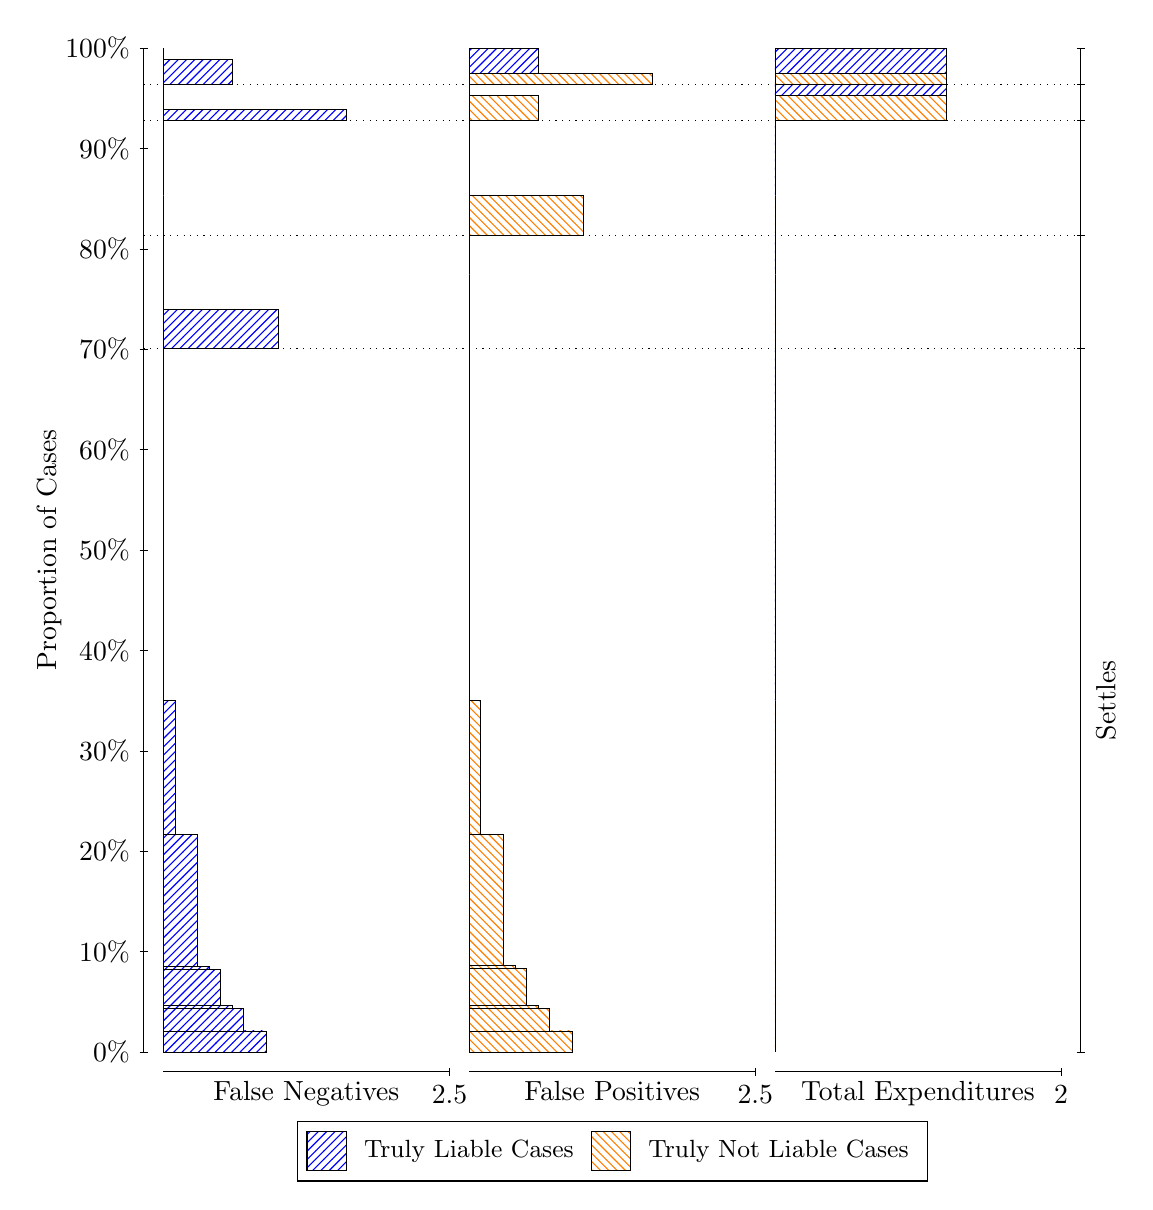
\begin{tikzpicture}
\draw[black, very thin] (1.5,1.75) -- (1.5,14.5);
\node[rotate=90, text=black, anchor=center] at (0.3, 8.125) {Proportion of Cases};
\draw[black, very thin] (1.45,1.75) -- (1.55,1.75);
\node[text=black, anchor=east] at (1.45, 1.75) {0\%};
\draw[black, very thin] (1.45,3.025) -- (1.55,3.025);
\node[text=black, anchor=east] at (1.45, 3.025) {10\%};
\draw[black, very thin] (1.45,4.3) -- (1.55,4.3);
\node[text=black, anchor=east] at (1.45, 4.3) {20\%};
\draw[black, very thin] (1.45,5.575) -- (1.55,5.575);
\node[text=black, anchor=east] at (1.45, 5.575) {30\%};
\draw[black, very thin] (1.45,6.85) -- (1.55,6.85);
\node[text=black, anchor=east] at (1.45, 6.85) {40\%};
\draw[black, very thin] (1.45,8.125) -- (1.55,8.125);
\node[text=black, anchor=east] at (1.45, 8.125) {50\%};
\draw[black, very thin] (1.45,9.4) -- (1.55,9.4);
\node[text=black, anchor=east] at (1.45, 9.4) {60\%};
\draw[black, very thin] (1.45,10.675) -- (1.55,10.675);
\node[text=black, anchor=east] at (1.45, 10.675) {70\%};
\draw[black, very thin] (1.45,11.95) -- (1.55,11.95);
\node[text=black, anchor=east] at (1.45, 11.95) {80\%};
\draw[black, very thin] (1.45,13.225) -- (1.55,13.225);
\node[text=black, anchor=east] at (1.45, 13.225) {90\%};
\draw[black, very thin] (1.45,14.5) -- (1.55,14.5);
\node[text=black, anchor=east] at (1.45, 14.5) {100\%};

\draw[black, very thin] (13.4,1.75) -- (13.4,14.5);
\draw[black, very thin] (13.35,1.75) -- (13.45,1.75);
\node[anchor=west] at (13.35, 1.75) {};
\draw[black, very thin] (13.35,10.682) -- (13.45,10.682);
\node[anchor=west] at (13.35, 10.682) {};
\draw[black, very thin] (13.35,12.124) -- (13.45,12.124);
\node[anchor=west] at (13.35, 12.124) {};
\draw[black, very thin] (13.35,13.578) -- (13.45,13.578);
\node[anchor=west] at (13.35, 13.578) {};
\draw[black, very thin] (13.35,14.042) -- (13.45,14.042);
\node[anchor=west] at (13.35, 14.042) {};
\draw[black, very thin] (13.35,14.5) -- (13.45,14.5);
\node[anchor=west] at (13.35, 14.5) {};

\draw[black, very thin, pattern color=blue, pattern=north east lines] (1.75,1.75) rectangle (3.058,2.0171);
\draw[black, very thin, pattern color=blue, pattern=north east lines] (1.75,2.0171) rectangle (2.7673,2.3016);
\draw[black, very thin, pattern color=blue, pattern=north east lines] (1.75,2.3016) rectangle (2.622,2.3412);
\draw[black, very thin, pattern color=blue, pattern=north east lines] (1.75,2.3412) rectangle (2.4767,2.8011);
\draw[black, very thin, pattern color=blue, pattern=north east lines] (1.75,2.8011) rectangle (2.3313,2.8407);
\draw[black, very thin, pattern color=blue, pattern=north east lines] (1.75,2.8407) rectangle (2.186,4.5177);
\draw[black, very thin, pattern color=blue, pattern=north east lines] (1.75,4.5177) rectangle (1.8953,6.2172);
\draw[black, very thin, pattern color=orange, pattern=north west lines] (1.75,6.2172) rectangle (1.75,10.682);
\draw[black, very thin, pattern color=blue, pattern=north east lines] (1.75,10.682) rectangle (3.2033,11.181);
\draw[black, very thin, pattern color=orange, pattern=north west lines] (1.75,11.181) rectangle (1.75,12.124);
\draw[black, very thin, pattern color=orange, pattern=north west lines] (1.75,12.124) rectangle (1.75,12.628);
\draw[black, very thin, pattern color=blue, pattern=north east lines] (1.75,12.628) rectangle (1.75,13.578);
\draw[black, very thin, pattern color=blue, pattern=north east lines] (1.75,13.578) rectangle (4.0753,13.719);
\draw[black, very thin, pattern color=orange, pattern=north west lines] (1.75,13.719) rectangle (1.75,14.042);
\draw[black, very thin, pattern color=blue, pattern=north east lines] (1.75,14.042) rectangle (2.622,14.36);
\draw[black, very thin, pattern color=orange, pattern=north west lines] (1.75,14.36) rectangle (1.75,14.5);
\draw[black, very thin, pattern color=orange, pattern=north west lines] (5.6333,1.75) rectangle (6.9413,2.0171);
\draw[black, very thin, pattern color=orange, pattern=north west lines] (5.6333,2.0171) rectangle (6.6507,2.3058);
\draw[black, very thin, pattern color=orange, pattern=north west lines] (5.6333,2.3058) rectangle (6.5053,2.3454);
\draw[black, very thin, pattern color=orange, pattern=north west lines] (5.6333,2.3454) rectangle (6.36,2.8076);
\draw[black, very thin, pattern color=orange, pattern=north west lines] (5.6333,2.8076) rectangle (6.2147,2.8472);
\draw[black, very thin, pattern color=orange, pattern=north west lines] (5.6333,2.8472) rectangle (6.0693,4.5155);
\draw[black, very thin, pattern color=orange, pattern=north west lines] (5.6333,4.5155) rectangle (5.7787,6.215);
\draw[black, very thin, pattern color=blue, pattern=north east lines] (5.6333,6.215) rectangle (5.6333,10.682);
\draw[black, very thin, pattern color=orange, pattern=north west lines] (5.6333,10.682) rectangle (5.6333,11.626);
\draw[black, very thin, pattern color=blue, pattern=north east lines] (5.6333,11.626) rectangle (5.6333,12.124);
\draw[black, very thin, pattern color=orange, pattern=north west lines] (5.6333,12.124) rectangle (7.0867,12.628);
\draw[black, very thin, pattern color=blue, pattern=north east lines] (5.6333,12.628) rectangle (5.6333,13.578);
\draw[black, very thin, pattern color=orange, pattern=north west lines] (5.6333,13.578) rectangle (6.5053,13.901);
\draw[black, very thin, pattern color=blue, pattern=north east lines] (5.6333,13.901) rectangle (5.6333,14.042);
\draw[black, very thin, pattern color=orange, pattern=north west lines] (5.6333,14.042) rectangle (7.9587,14.182);
\draw[black, very thin, pattern color=blue, pattern=north east lines] (5.6333,14.182) rectangle (6.5053,14.5);
\draw[black, very thin, pattern color=orange, pattern=north west lines] (9.5167,1.75) rectangle (9.5167,6.215);
\draw[black, very thin, pattern color=blue, pattern=north east lines] (9.5167,6.215) rectangle (9.5167,10.682);
\draw[black, very thin, pattern color=orange, pattern=north west lines] (9.5167,10.682) rectangle (9.5167,11.626);
\draw[black, very thin, pattern color=blue, pattern=north east lines] (9.5167,11.626) rectangle (9.5167,12.124);
\draw[black, very thin, pattern color=orange, pattern=north west lines] (9.5167,12.124) rectangle (9.5167,12.628);
\draw[black, very thin, pattern color=blue, pattern=north east lines] (9.5167,12.628) rectangle (9.5167,13.578);
\draw[black, very thin, pattern color=orange, pattern=north west lines] (9.5167,13.578) rectangle (11.697,13.901);
\draw[black, very thin, pattern color=blue, pattern=north east lines] (9.5167,13.901) rectangle (11.697,14.042);
\draw[black, very thin, pattern color=orange, pattern=north west lines] (9.5167,14.042) rectangle (11.697,14.182);
\draw[black, very thin, pattern color=blue, pattern=north east lines] (9.5167,14.182) rectangle (11.697,14.5);
\draw[black, dotted] (1.5,10.682) -- (13.4,10.682);
\draw[black, dotted] (1.5,12.124) -- (13.4,12.124);
\draw[black, dotted] (1.5,13.578) -- (13.4,13.578);
\draw[black, dotted] (1.5,14.042) -- (13.4,14.042);
\draw[black, very thin] (1.75,1.5) -- (5.3833,1.5);
\node[text=black, anchor=north] at (3.5667, 1.5) {False Negatives};
\draw[black, very thin] (5.3833,1.45) -- (5.3833,1.55);
\node[text=black, anchor=north] at (5.3833, 1.45) {2.5};

\draw[black, very thin] (5.6333,1.5) -- (9.2667,1.5);
\node[text=black, anchor=north] at (7.45, 1.5) {False Positives};
\draw[black, very thin] (9.2667,1.45) -- (9.2667,1.55);
\node[text=black, anchor=north] at (9.2667, 1.45) {2.5};

\draw[black, very thin] (9.5167,1.5) -- (13.15,1.5);
\node[text=black, anchor=north] at (11.333, 1.5) {Total Expenditures};
\draw[black, very thin] (13.15,1.45) -- (13.15,1.55);
\node[text=black, anchor=north] at (13.15, 1.45) {2};

\node[text=black, centered, rotate=90] at (13.72, 6.2161) {Settles};





\draw (7.449999999999999,1.5) node[draw=none] (baseCoordinate) {};
\begin{scope}[align=center]
        \matrix[scale=0.5, draw=black, below=0.5cm of baseCoordinate, nodes={draw}, column sep=0.1cm]{
            \node[rectangle, draw, minimum width=0.5cm, minimum height=0.5cm, pattern color=blue, pattern=north east lines] {}; &
            \node[draw=none, font=\small, text=black] (B) {Truly Liable Cases}; &
            \node[rectangle, draw, minimum width=0.5cm, minimum height=0.5cm, pattern color=orange, pattern=north west lines] {}; &
            \node[draw=none, font=\small, text=black] (B) {Truly Not Liable Cases}; \\
            };
\end{scope}

\end{tikzpicture}
\end{document}